% !TEX program = xelatex
% !TEX encoding = UTF-8 Unicode
% =====================================================================
%  Homework 3.2 — Data Warehouse Design (Star Schema)
%  Case study: "Culture Passport" (หนังสือเดินทางวัฒนธรรม)
%  MUST compile with XeLaTeX (Thai fonts). Monochrome / grayscale theme.
% =====================================================================
\documentclass[11pt]{article}

\usepackage{fontspec}
\usepackage[a4paper,margin=2cm]{geometry}
\usepackage{underscore}                 % lets snake_case print literally
\usepackage{tikz}
\usetikzlibrary{positioning,shapes.multipart,arrows.meta,fit,backgrounds}
\usepackage{xcolor}
\usepackage{booktabs}
\usepackage{tabularx}
\usepackage{array}
\usepackage{colortbl}
\usepackage{multirow}
\usepackage{enumitem}
\usepackage{fancyhdr}
\usepackage{fancyvrb}
\usepackage{caption}
\usepackage{graphicx}
\usepackage{adjustbox}        % shrink wide sample tables to page width
\usepackage[hidelinks]{hyperref}

% ---- Fonts (ONE font for everything: Thai + Latin + code + SQL) ------
\setmainfont{Waree}          % TLWG dual-script: full Latin + Thai, has Bold/Italic
\setmonofont{Waree}          % same font for \texttt/\code and SQL (fancyvrb) blocks

% Enable ICU dictionary-based Thai line breaking (Thai has no spaces between words)
\XeTeXlinebreaklocale "th"
\XeTeXlinebreakskip = 0pt plus 0.1em minus 0.05em

% ---- Colours (MONOCHROME / grayscale theme) --------------------------
\definecolor{factHead}{gray}{0.18}   % darkest gray — Fact header, section & main titles
\definecolor{factBody}{gray}{0.90}   % light gray — Fact body fill
\definecolor{dimHead}{gray}{0.40}    % medium gray — Dimension headers
\definecolor{dimBody}{gray}{0.95}    % very light gray — Dimension body fill
\definecolor{tblHead}{gray}{0.28}    % dark gray — table header bands
\definecolor{tblAlt}{gray}{0.93}     % light gray — zebra alternate rows
\definecolor{accent}{gray}{0.00}     % black — PK marker
\definecolor{codeframe}{gray}{0.55}  % gray — SQL frame rule

% ---- Header / footer -------------------------------------------------


% ---- Helpers ---------------------------------------------------------
\newcommand{\code}[1]{\texttt{#1}}
\newcommand{\PK}{\textbf{\textcolor{accent}{PK}}}
\newcommand{\FK}{\textbf{\textcolor{factHead}{FK}}}
\newcommand{\secline}{\par\vspace{-2pt}\noindent\textcolor{tblHead}{\rule{\linewidth}{0.8pt}}\par\vspace{3pt}}

% Section styling
\usepackage{titlesec}
\titleformat{\section}{\large\bfseries\color{factHead}}{\thesection.}{0.5em}{}
\titlespacing*{\section}{0pt}{8pt}{4pt}

% SQL block style
\DefineVerbatimEnvironment{sql}{Verbatim}%
  {fontsize=\footnotesize,frame=single,framesep=5pt,rulecolor=\color{codeframe},%
   xleftmargin=4pt,xrightmargin=4pt}

\newcolumntype{Y}{>{\raggedright\arraybackslash}X}

% Attribute-table header row (3 columns: Attribute / Type / Description)
\newcommand{\atthead}{\rowcolor{tblHead}
  \textcolor{white}{\textbf{Attribute}} & \textcolor{white}{\textbf{Type}} & \textcolor{white}{\textbf{Description}}\\}

\begin{document}

% =====================================================================
% TITLE BLOCK
% =====================================================================

% =====================================================================
\section{Business Process, Granularity, Dimensions, Measures}
% =====================================================================
\begin{description}[leftmargin=0pt,itemsep=1pt,topsep=1pt]
  \item[Business Process:] การเข้าร่วมกิจกรรมของสมาชิก (Member Activity Participation)
  \item[Granularity:] 1 แถว = สมาชิก 1 คน เข้าร่วมกิจกรรม 1 รอบ (atomic grain)
  \item[Dimensions (5):] \code{Dim_Date} (เวลา/ฤดู/เทศกาล), \code{Dim_Member} (ผู้เข้าร่วม + ระดับสมาชิก),
        \code{Dim_Activity} (กิจกรรม/ประเภท), \code{Dim_Location} (สถานที่/ภูมิภาค), \code{Dim_Team} (ทีมงาน)
  \item[Measures:] \code{amount_paid}, \code{discount_amount}, \code{points_earned}, \code{participant_count}
        (additive); \code{review_score} (non-additive $\to$ ใช้ \code{AVG})
\end{description}

\vspace{6pt}
% =====================================================================
\section{ผัง Star Schema}
% =====================================================================
\vspace{6pt}
\begin{center}
\resizebox{0.92\linewidth}{!}{%
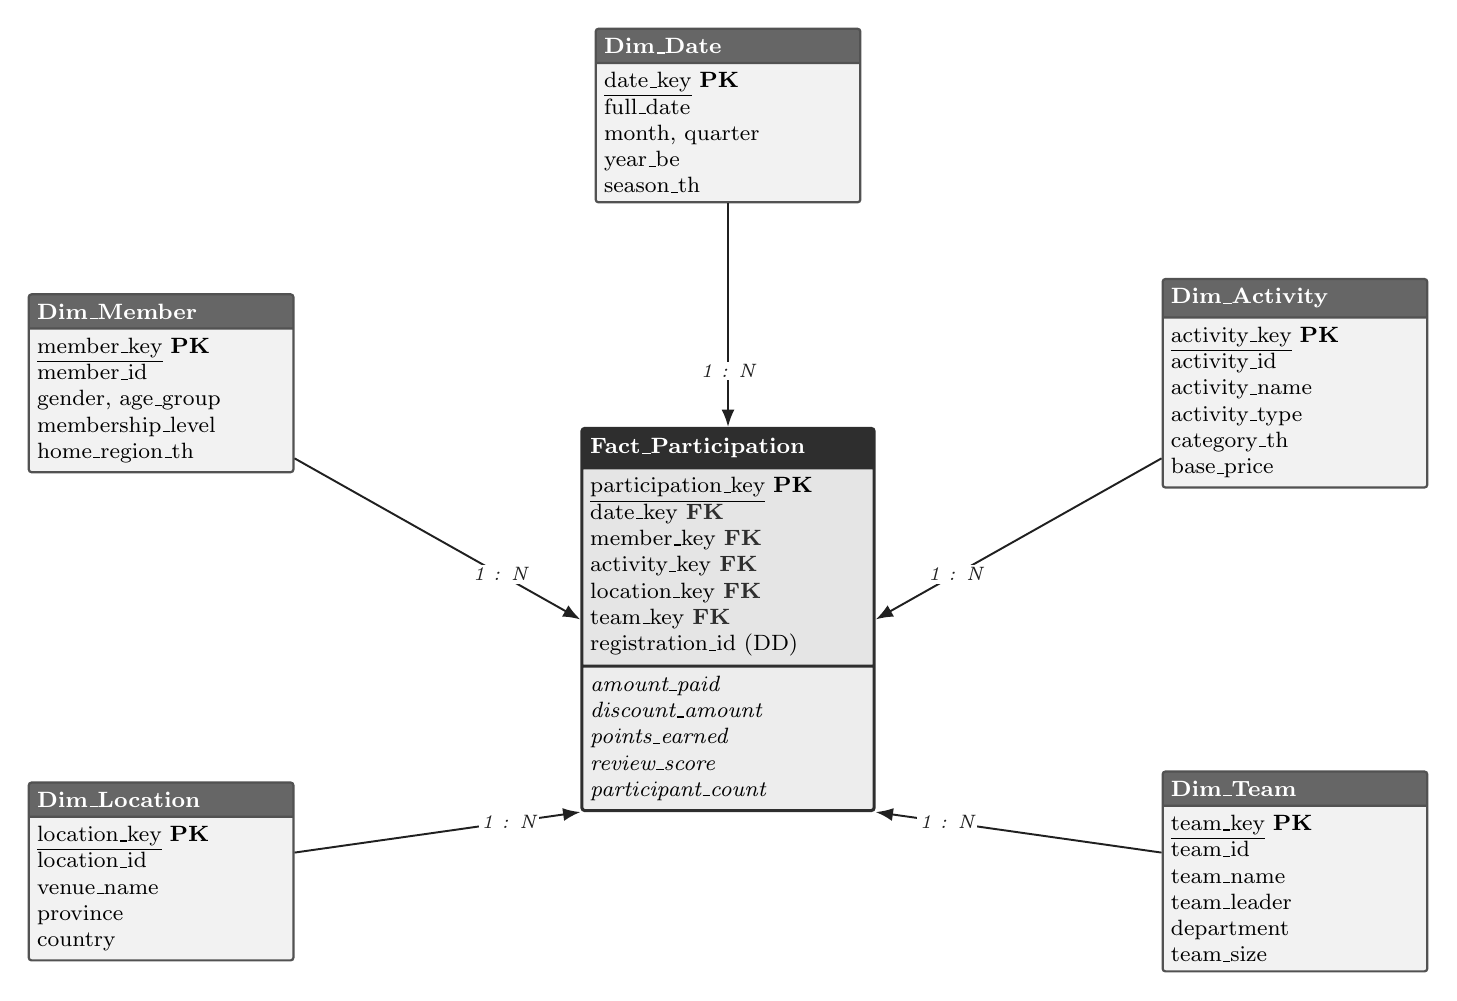
\begin{tikzpicture}[
  every node/.style={font=\footnotesize},
  tbl/.style={draw=dimHead!80!black, line width=0.8pt, rounded corners=1pt,
      rectangle split, rectangle split parts=2,
      rectangle split part fill={dimHead, dimBody},
      text width=3.15cm, align=left, inner sep=3pt},
  facttbl/.style={draw=factHead, line width=1.1pt, rounded corners=1pt,
      rectangle split, rectangle split parts=3,
      rectangle split part fill={factHead, factBody, factBody!70!white},
      text width=3.5cm, align=left, inner sep=3pt},
  rel/.style={-{Latex[length=2.2mm]}, line width=0.7pt, factHead!70!black},
  hdr/.style={text=white},
  lbl/.style={font=\scriptsize\itshape, fill=white, inner sep=1pt}
]
\node[facttbl] (fact) at (0,0) {
  \nodepart[hdr]{one}\textbf{Fact_Participation}
  \nodepart{two}
    \underline{participation_key} \PK\\
    date_key \FK\\ member_key \FK\\ activity_key \FK\\
    location_key \FK\\ team_key \FK\\ registration_id (DD)
  \nodepart{three}
    \textit{amount_paid}\\ \textit{discount_amount}\\
    \textit{points_earned}\\ \textit{review_score}\\ \textit{participant_count}
};
\node[tbl] (date) at (0,6.4) {
  \nodepart[hdr]{one}\textbf{Dim_Date}
  \nodepart{two}\underline{date_key} \PK\\ full_date\\ month, quarter\\ year_be\\ season_th};
\node[tbl] (member) at (-7.2,3.0) {
  \nodepart[hdr]{one}\textbf{Dim_Member}
  \nodepart{two}\underline{member_key} \PK\\ member_id\\ gender, age_group\\ membership_level\\ home_region_th};
\node[tbl] (activity) at (7.2,3.0) {
  \nodepart[hdr]{one}\textbf{Dim_Activity}
  \nodepart{two}\underline{activity_key} \PK\\ activity_id\\ activity_name\\ activity_type\\ category_th\\ base_price};
\node[tbl] (location) at (-7.2,-3.2) {
  \nodepart[hdr]{one}\textbf{Dim_Location}
  \nodepart{two}\underline{location_key} \PK\\ location_id\\ venue_name\\ province\\ country};
\node[tbl] (team) at (7.2,-3.2) {
  \nodepart[hdr]{one}\textbf{Dim_Team}
  \nodepart{two}\underline{team_key} \PK\\ team_id\\ team_name\\ team_leader\\ department\\ team_size};
\draw[rel] (date)     -- node[lbl,pos=0.75]{1 : N} (fact.north);
\draw[rel] (member)   -- node[lbl,pos=0.72]{1 : N} (fact.west);
\draw[rel] (activity) -- node[lbl,pos=0.72]{1 : N} (fact.east);
\draw[rel] (location) -- node[lbl,pos=0.75]{1 : N} (fact.south west);
\draw[rel] (team)     -- node[lbl,pos=0.75]{1 : N} (fact.south east);
\end{tikzpicture}}
\end{center}
\clearpage

% =====================================================================
\section{คำอธิบาย Attribute }
% =====================================================================
\small
\subsection*{Dim_Date}
\begin{tabularx}{\linewidth}{@{}l l Y@{}}
\toprule \atthead \midrule
\code{date_key} & INT & PK - YYYYMMDD\\
\code{full_date} & DATE & วันที่จัดกิจกรรม\\
\code{month} & INT & เดือน \\
\code{quarter} & INT & ไตรมาส\\
\code{year_be} & INT & ปี พ.ศ.\\
\code{season_th} & VARCHAR(15) & ฤดูกาล: ร้อน, ฝน, หนาว\\
\bottomrule
\end{tabularx}

\subsection*{Dim_Member}
\begin{tabularx}{\linewidth}{@{}l l Y@{}}
\toprule \atthead \midrule
\code{member_key} & INT & PK \\
\code{member_id} & VARCHAR(10) & รหัสสมาชิกต้นทาง\\
\code{gender} & CHAR(1) & เพศ \\
\code{age_group} & VARCHAR(10) & ช่วงอายุ\\
\code{is_foreigner} & BOOLEAN & แยกไทย, ต่างชาติ\\
\code{membership_level} & VARCHAR(10) & ระดับ: Silver, Gold, Platinum\\
\code{home_region_th} & VARCHAR(15) & ภูมิภาคที่อยู่อาศัย\\
\bottomrule
\end{tabularx}

\subsection*{Dim_Activity}
\begin{tabularx}{\linewidth}{@{}l l Y@{}}
\toprule \atthead \midrule
\code{activity_key} & INT & PK \\
\code{activity_id} & VARCHAR(10) & รหัสกิจกรรมต้นทาง\\
\code{activity_name} & VARCHAR(150) & ชื่อกิจกรรม\\
\code{activity_type} & VARCHAR(40) & ประเภท: Temple Tour, Workshop, Camp, Local Life\\
\code{category_th} & VARCHAR(30) & หมวดหมู่\\
\code{base_price} & DECIMAL(10,2) & ราคาต่อคน (บาท)\\
\bottomrule
\end{tabularx}

\subsection*{Dim_Location}
\begin{tabularx}{\linewidth}{@{}l l Y@{}}
\toprule \atthead \midrule
\code{location_key} & INT & PK \\
\code{location_id} & VARCHAR(10) & รหัสสถานที่ต้นทาง\\
\code{venue_name} & VARCHAR(100) & ชื่อสถานที่\\
\code{province} & VARCHAR(30) & จังหวัด\\
\code{country} & VARCHAR(30) & ประเทศ\\
\bottomrule
\end{tabularx}

\subsection*{Dim_Team}
\begin{tabularx}{\linewidth}{@{}l l Y@{}}
\toprule \atthead \midrule
\code{team_key} & INT & PK \\
\code{team_id} & VARCHAR(10) & รหัสทีมต้นทาง\\
\code{team_name} & VARCHAR(60) & ชื่อทีม\\
\code{team_leader} & VARCHAR(60) & หัวหน้าทีม\\
\code{department} & VARCHAR(40) & แผนก\\
\code{team_size} & INT & จำนวนสมาชิกในทีม\\
\bottomrule
\end{tabularx}

\subsection*{Fact_Participation}
\begin{tabularx}{\linewidth}{@{}l l Y@{}}
\toprule \atthead \midrule
\code{participation_key} & BIGINT & PK\\
\code{date_key} & INT & FK \\
\code{member_key} & INT & FK\\
\code{activity_key} & INT & FK \\
\code{location_key} & INT & FK \\
\code{team_key} & INT & FK \\
\code{registration_id} & VARCHAR(15) & เลขที่ใบลงทะเบียน\\
\code{amount_paid} & DECIMAL(10,2) & ค่าใช้จ่ายที่ชำระ \\
\code{discount_amount} & DECIMAL(10,2) & ส่วนลด \\
\code{points_earned} & INT & คะแนนสะสม \\
\code{review_score} & DECIMAL(2,1) & คะแนนรีวิว\\
\code{participant_count} & INT & 1 ต่อแถว \\
\bottomrule
\end{tabularx}
\normalsize

% =====================================================================
\section{ตัวอย่างข้อมูล }
% =====================================================================
\footnotesize
\subsection*{Dim_Date}
\begin{adjustbox}{max width=\linewidth}
\begin{tabular}{@{}l l c c c l@{}}
\toprule
\rowcolor{tblHead}\textcolor{white}{date_key} & \textcolor{white}{full_date} & \textcolor{white}{month} & \textcolor{white}{quarter} & \textcolor{white}{year_be} & \textcolor{white}{season_th}\\
\midrule
20240413 & 2024-04-13 & 4 & 2 & 2567 & ฤดูร้อน\\
20240414 & 2024-04-14 & 4 & 2 & 2567 & ฤดูร้อน\\
20240705 & 2024-07-05 & 7 & 3 & 2567 & ฤดูฝน\\
20241115 & 2024-11-15 & 11 & 4 & 2567 & ฤดูหนาว\\
20250118 & 2025-01-18 & 1 & 1 & 2568 & ฤดูหนาว\\
20250412 & 2025-04-12 & 4 & 2 & 2568 & ฤดูร้อน\\
\bottomrule
\end{tabular}
\end{adjustbox}

\subsection*{Dim_Member}
\begin{adjustbox}{max width=\linewidth}
\begin{tabular}{@{}c l c l c l l@{}}
\toprule
\rowcolor{tblHead}\textcolor{white}{member_key} & \textcolor{white}{member_id} & \textcolor{white}{gender} & \textcolor{white}{age_group} & \textcolor{white}{is_foreigner} & \textcolor{white}{membership_level} & \textcolor{white}{home_region_th}\\
\midrule
1 & CP-0001 & M & 36-45 & FALSE & Platinum & ภาคกลาง\\
2 & CP-0002 & F & 25-35 & TRUE & Gold & -\\
3 & CP-0003 & F & 46-55 & FALSE & Platinum & ภาคอีสาน\\
4 & CP-0004 & M & 36-45 & TRUE & Silver & -\\
5 & CP-0005 & M & 18-24 & FALSE & Gold & ภาคเหนือ\\
6 & CP-0006 & F & 25-35 & FALSE & Platinum & ภาคใต้\\
\bottomrule
\end{tabular}
\end{adjustbox}

\subsection*{Dim_Activity}
\begin{adjustbox}{max width=\linewidth}
\begin{tabular}{@{}c l l l l r@{}}
\toprule
\rowcolor{tblHead}\textcolor{white}{activity_key} & \textcolor{white}{activity_id} & \textcolor{white}{activity_name} & \textcolor{white}{activity_type} & \textcolor{white}{category_th} & \textcolor{white}{base_price}\\
\midrule
1 & ACT-01 & ทัวร์วัดพระแก้วและพระบรมมหาราชวัง & Temple Tour & มรดกวัฒนธรรม & 500.00\\
2 & ACT-02 & เวิร์กช็อปเครื่องปั้นดินเผาบ้านเชียง & Art Workshop & หัตถกรรม & 800.00\\
3 & ACT-03 & ค่ายวัฒนธรรมอีสานสามวันสองคืน & Cultural Camp & วิถีชุมชน & 3500.00\\
4 & ACT-04 & เรียนรู้วิถีชีวิตชาวนาล้านนา & Local Life & วิถีชุมชน & 600.00\\
5 & ACT-05 & เวิร์กช็อปผ้าบาติกภาคใต้ & Art Workshop & หัตถกรรม & 900.00\\
\bottomrule
\end{tabular}
\end{adjustbox}

\subsection*{Dim_Location}
\begin{adjustbox}{max width=\linewidth}
\begin{tabular}{@{}c l l l l@{}}
\toprule
\rowcolor{tblHead}\textcolor{white}{location_key} & \textcolor{white}{location_id} & \textcolor{white}{venue_name} & \textcolor{white}{province} & \textcolor{white}{country}\\
\midrule
1 & LOC-01 & วัดพระศรีรัตนศาสดาราม & กรุงเทพมหานคร & Thailand\\
2 & LOC-02 & แหล่งโบราณคดีบ้านเชียง & อุดรธานี & Thailand\\
3 & LOC-03 & หมู่บ้านวัฒนธรรมอีสาน & ขอนแก่น & Thailand\\
4 & LOC-04 & เมืองเก่าเชียงใหม่ & เชียงใหม่ & Thailand\\
5 & LOC-05 & ย่านเมืองเก่าภูเก็ต & ภูเก็ต & Thailand\\
\bottomrule
\end{tabular}
\end{adjustbox}

\subsection*{Dim_Team}
\begin{adjustbox}{max width=\linewidth}
\begin{tabular}{@{}c l l l l c@{}}
\toprule
\rowcolor{tblHead}\textcolor{white}{team_key} & \textcolor{white}{team_id} & \textcolor{white}{team_name} & \textcolor{white}{team_leader} & \textcolor{white}{department} & \textcolor{white}{team_size}\\
\midrule
1 & TM-01 & ทีมมรดกกรุงเทพ & อนันต์ ประเสริฐ & Heritage Operations & 5\\
2 & TM-02 & ทีมศิลป์ถิ่นอีสาน & พลอย ศรีสุข & Workshop Operations & 4\\
3 & TM-03 & ทีมล้านนาสร้างสรรค์ & กิตติ วงศ์คำ & Community Operations & 6\\
4 & TM-04 & ทีมอันดามัน & มณี ทะเลใส & Workshop Operations & 4\\
\bottomrule
\end{tabular}
\end{adjustbox}

\subsection*{Fact_Participation (12 แถว)}
\begin{adjustbox}{max width=\linewidth}
\begin{tabular}{@{}c c c c c c l r r r c c@{}}
\toprule
\rowcolor{tblHead}
\textcolor{white}{participation_key} & \textcolor{white}{date_key} & \textcolor{white}{member_key} & \textcolor{white}{activity_key} & \textcolor{white}{location_key} & \textcolor{white}{team_key} & \textcolor{white}{registration_id} & \textcolor{white}{amount_paid} & \textcolor{white}{discount_amount} & \textcolor{white}{points_earned} & \textcolor{white}{review_score} & \textcolor{white}{participant_count}\\
\midrule
1 & 20240413 & 1 & 1 & 1 & 1 & REG-100001 & 500.00 & 0.00 & 50 & 4.5 & 1\\
2 & 20240413 & 2 & 1 & 1 & 1 & REG-100002 & 500.00 & 0.00 & 50 & 5.0 & 1\\
3 & 20240414 & 6 & 1 & 1 & 1 & REG-100003 & 450.00 & 50.00 & 45 & 4.0 & 1\\
4 & 20240414 & 4 & 2 & 2 & 2 & REG-100004 & 720.00 & 80.00 & 80 & 4.0 & 1\\
5 & 20240705 & 3 & 3 & 3 & 2 & REG-100005 & 3150.00 & 350.00 & 300 & 4.5 & 1\\
6 & 20240705 & 5 & 3 & 3 & 2 & REG-100006 & 3500.00 & 0.00 & 350 & 3.5 & 1\\
7 & 20241115 & 1 & 4 & 4 & 3 & REG-100007 & 600.00 & 0.00 & 60 & 5.0 & 1\\
8 & 20241115 & 5 & 4 & 4 & 3 & REG-100008 & 600.00 & 0.00 & 60 & 4.5 & 1\\
9 & 20250118 & 6 & 5 & 5 & 4 & REG-100009 & 900.00 & 0.00 & 90 & 4.0 & 1\\
10 & 20250118 & 2 & 5 & 5 & 4 & REG-100010 & 810.00 & 90.00 & 90 & 4.5 & 1\\
11 & 20250412 & 1 & 1 & 1 & 1 & REG-100011 & 500.00 & 0.00 & 50 & 4.5 & 1\\
12 & 20250412 & 3 & 2 & 2 & 2 & REG-100012 & 800.00 & 0.00 & 80 & 5.0 & 1\\
\bottomrule
\end{tabular}
\end{adjustbox}
\normalsize
\clearpage
% =====================================================================
\section{Business Questions}
% =====================================================================
\textbf{Q1.} จำนวนผู้เข้าร่วมกิจกรรมแยกตามประเภทกิจกรรมในปี 2567
\begin{sql}
SELECT a.activity_type, COUNT(*) AS n_participants
FROM Fact_Participation f
JOIN Dim_Activity a ON f.activity_key=a.activity_key
JOIN Dim_Date d ON f.date_key=d.date_key
WHERE d.year_be=2567
GROUP BY a.activity_type;
\end{sql}


\textbf{Q2.} ทีมงานที่ได้คะแนนรีวิวสูงสุดแยกตามปี
\begin{sql}
SELECT d.year_be, t.team_name, AVG(f.review_score) AS avg_review
FROM Fact_Participation f
JOIN Dim_Team t ON f.team_key=t.team_key
JOIN Dim_Date d ON f.date_key=d.date_key
GROUP BY d.year_be, t.team_name
ORDER BY d.year_be, avg_review DESC;
\end{sql}

\textbf{Q3.} ผู้เข้าร่วมกิจกรรมที่ได้รับคะแนนสะสมสูงสุดในแต่ละภูมิภาค
\begin{sql}
SELECT m.home_region_th, m.member_id, SUM(f.points_earned) AS total_points
FROM Fact_Participation f
JOIN Dim_Member m ON f.member_key=m.member_key
GROUP BY m.home_region_th, m.member_id
ORDER BY m.home_region_th, total_points DESC;
\end{sql}

\textbf{Q4.} ฤดูใดมีรายได้รวมสูงสุดจากกิจกรรมประเภท Art Workshop
\begin{sql}
SELECT d.season_th, SUM(f.amount_paid) AS total_revenue
FROM Fact_Participation f
JOIN Dim_Activity a ON f.activity_key=a.activity_key
JOIN Dim_Date d ON f.date_key=d.date_key
WHERE a.activity_type='Art Workshop'
GROUP BY d.season_th ORDER BY total_revenue DESC;
\end{sql}

\textbf{Q5.} รายได้ที่ได้รับแยกคนในประเทศไทย/ต่างชาติ
\begin{sql}
SELECT m.is_foreigner, SUM(f.amount_paid) AS total_revenue
FROM Fact_Participation f
JOIN Dim_Member m ON f.member_key=m.member_key
GROUP BY m.is_foreigner;
\end{sql}

\end{document}
